\section{Data}
\label{sec:formatting}

\subsection{Data Sources}

This project integrates data from the two main sources:
\begin{itemize}

  \item \textbf{Lakh MIDI Dataset (LMD)}\cite{raffel2016lakh} - A large-scale collection of MIDI files (machine-readable representation of musical structure) representing music in symbolic form (notes, timing, instruments.
  \item \textbf{Million Song Dataset (MSD)}\cite{msd2011}\cite{echonest2011} - A dataset developed by The Echo Nest, containing audio-derived features such as tempo, key, or loudness metadata for songs, as well as a user taste profile subset.
\end{itemize}

\subsection{Data Processing}
The first step of the data processing methodology involved the extraction and linking of the Lakh MIDI and Million Song Dataset (MSD). The alignment between MIDI files and audio tracks was based on precomputed similarity scores obtained using Dynamic Time Warping (DTW) by Raffel (2016). In this process, both MIDI and audio signals were first converted into chroma-based representations over time, and then compared to determine their similarity. The threshold for acceptable similarity score of 0.55 was set during the filtering step, in order to ensure reliable alignment. The remaining files and duplicates were omitted resulting in a dataset of 19,037 tracks, with each one described at this stage by 40 metadata fields which included track-level identifiers (e.g. track\_id, song\_id, or artist\_id), descriptive fields (e.g. title, artist name, album, release year), tonal estimates (key, mode, and their confidences), rhythmic/audio scalars (time signature, loudness), genre/tag information (e.g. primary genre, top-3 genres), and MIDI-derived instrumentation (number and names of instruments). The exploratory overview of the MSD features is available in Figure ~\ref{fig:MSD_features} of the Appendix.

The next step concerned processing and subsequently linking user interaction data extracted from Echo Nest Taste Profile, represented in the form of \mbox{(\texttt{user\_id}, \texttt{song\_id}, \texttt{play\_count})} triplets. The raw dataset consisted of approximately 48 million interactions across over one million users and almost four hundred thousand songs. Interactions associated with known erroneous song ID mappings were removed using the official MSD mismatch list, which identified 18,913 incorrectly linked song IDs, of which 6,237 were present in the taste profile, accounting for 5.33\% of all interactions. Subsequently, the user data was filtered to retain only the songs that also exist in the Lakh/MSD previously matched dataset, which constituted approximately 40.4\% of all LMD songs. Additionally, instances with fewer than 5 remaining song interactions were removed to address the cold start problem, excluding users with insufficient listening history to train and evaluate recommendations for them. After the filtering step the dataset consisted of 299,156 unique users and 7,227 unique songs. Figure~\ref{fig:taste_profile} illustrates the filtering funnel across three dimensions: total interactions, unique users, and unique songs, at each step of the filtering pipeline. 

\begin{figure}[H]
    \centering
    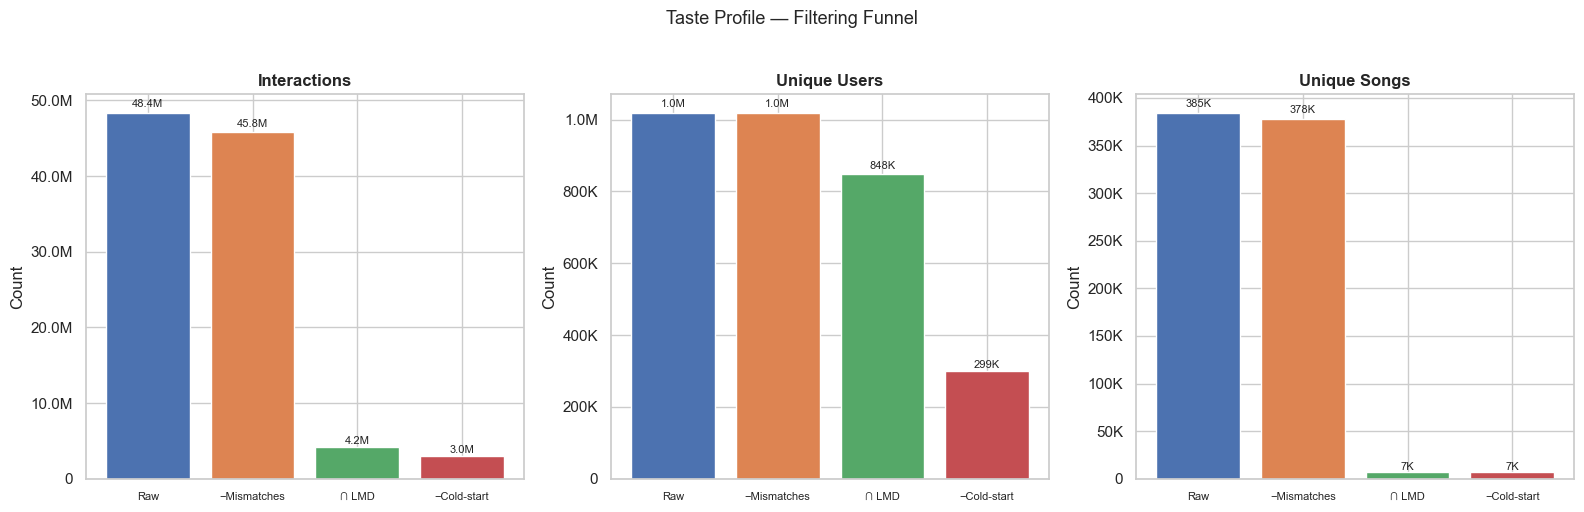
\includegraphics[width=0.75\linewidth]{sec/figures/taste_profile_graph.png}
    \caption{Taste Profile filtering funnel.}
    \label{fig:taste_profile}
\end{figure}

The detailed filtering statistics across all steps, together with filtered dataset diagnostics are summarized in Table ~\ref{tab:data_filtering} and ~\ref{fig:user_diagnostics} of the Appendix.

After the data integration and filtering process, feature extraction was performed using the jSymbolic~\cite{mckay2018jsymbolic} and music21~\cite{music21docs} extractors, which work directly with symbolic MIDI representations and produce high-level descriptors grounded in music theory. Out of the 19,037 matched tracks, 7,013 were successfully processed, forming the basis for all downstream modelling.

For each track jSymbolic and music21 together produced 1,525 numerical descriptors spanning seven categories: \textbf{pitch} (histograms, range, most-common-pitch statistics), \textbf{melodic} (interval histograms, arc direction and length), \textbf{harmonic} (simultaneous pitch distances), \textbf{rhythmic} (beat histograms, tempo statistics, note density), \textbf{dynamics} (loudness range, note-to-note variation), \textbf{textural} (voice count, voice equality), and \textbf{instrumentation}. The high dimensionality arises primarily from multi-bin histogram descriptors; the remaining features were approximately 150 scalars per track.
